\documentclass{amsart}

\usepackage{graphicx}
\usepackage{booktabs}
\begin{document}

\begin{table}[htbp]
\caption{Bias with minimum $\chi^2$  for different $\ell_{max}$ using 25 $\ell$'s per bin.}
\centering
\begin{tabular}{p{0.18\textwidth}p{0.18\textwidth}p{0.18\textwidth}p{0.18\textwidth}p{0.18\textwidth}p{0.18\textwidth}} \\ \toprule
$\ell_{max}$ & \multicolumn{1}{p{0cm}}{$b_{QSO}$} & $b_{DLA}$ & \multicolumn{1}{p{2cm}}{$\chi^2$} & d.o.f  & Probability\\ \midrule
300  &  2.9  $\pm$  0.66  &  1.31  $\pm$  1.37  &  15.49  &  22  &  0.16 \\
600  &  2.59  $\pm$  0.49  &  2.25  $\pm$  1.18  &  34.83  &  46  &  0.11 \\
900  &  2.61  $\pm$  0.46  &  2.26  $\pm$  1.15  &  66.89  &  70  &  0.42 \\
1200  &  2.67  $\pm$  0.46  &  2.19  $\pm$  1.14  &  92.05  &  94  &  0.46 \\
1500  &  2.73  $\pm$  0.45  &  2.14  $\pm$  1.13  &  111.93  &  118  &  0.36 \\
1800  &  2.77  $\pm$  0.45  &  2.19  $\pm$  1.13  &  133.29  &  142  &  0.31 \\
2100  &  2.8  $\pm$  0.45  &  2.17  $\pm$  1.13  &  152.57  &  166  &  0.24 \\ \bottomrule
\end{tabular}
\end{table}


\begin{table}[htbp]
\caption{Bias with minimum $\chi^2$  for different $\ell_{max}$ using 50 $\ell$'s per bin.}
\centering
\begin{tabular}{p{0.18\textwidth}p{0.18\textwidth}p{0.18\textwidth}p{0.18\textwidth}p{0.18\textwidth}p{0.18\textwidth}} \\ \toprule
$\ell_{max}$ & \multicolumn{1}{p{0cm}}{$b_{QSO}$} & $b_{DLA}$ & \multicolumn{1}{p{2cm}}{$\chi^2$} & d.o.f  & Probability\\ \midrule
300 & 2.75 $\pm$ 0.73 & 1.95 $\pm$ 1.44 & 12.37 & 10 & 0.74 \\
600 & 2.58 $\pm$ 0.49 & 2.62 $\pm$ 1.19 & 21.92 & 22 & 0.54 \\
900 & 2.61 $\pm$ 0.47& 2.7 $\pm$ 1.15 & 39.20 & 34 & 0.75  \\
1200  &  2.69  $\pm$  0.46  &  2.5  $\pm$  1.13  &  53.69  &  46  &  0.8 \\
1500  &  2.73  $\pm$  0.46  &  2.44  $\pm$  1.13  &  64.07  &  58  &  0.73 \\
1800  &  2.79  $\pm$  0.46  &  2.46  $\pm$  1.13  &  80.05  &  70  &  0.81 \\
2100  &  2.8  $\pm$  0.45  &  2.52  $\pm$  1.13  &  91.04  &  82  &  0.77 \\\bottomrule
\end{tabular}
\end{table}

\begin{table}[htbp]
\caption{Bias with minimum $\chi^2$  for different $\ell_{max}$ using 75 $\ell$'s per bin.}
\centering
\begin{tabular}{p{0.18\textwidth}p{0.18\textwidth}p{0.18\textwidth}p{0.18\textwidth}p{0.18\textwidth}p{0.18\textwidth}} \\ \toprule
$\ell_{max}$ & \multicolumn{1}{p{0cm}}{$b_{QSO}$} & $b_{DLA}$ & \multicolumn{1}{p{2cm}}{$\chi^2$} & d.o.f  & Probability\\ \midrule
300  &  3.36  $\pm$  0.83  &  1.66  $\pm$  1.61  &  9.83  &  6  &  0.87 \\
600  &  2.88  $\pm$  0.51  &  2.29  $\pm$  1.27  &  19.03  &  14  &  0.84 \\
900  &  2.82  $\pm$  0.47  &  2.71  $\pm$  1.21  &  31.25  &  22  &  0.91 \\
1200  &  2.85  $\pm$  0.46  &  2.56  $\pm$  1.19  &  44.24  &  30  &  0.95 \\
1500  &  2.9  $\pm$  0.46  &  2.42  $\pm$  1.19  &  53.2  &  38  &  0.95 \\
1800  &  2.96  $\pm$  0.46  &  2.47  $\pm$  1.19  &  62.25  &  46  &  0.94 \\
2100  &  2.96  $\pm$  0.45  &  2.54  $\pm$  1.18  &  69.14  &  54  &  0.92 \\ \bottomrule
\end{tabular}
\end{table}

\begin{figure}
  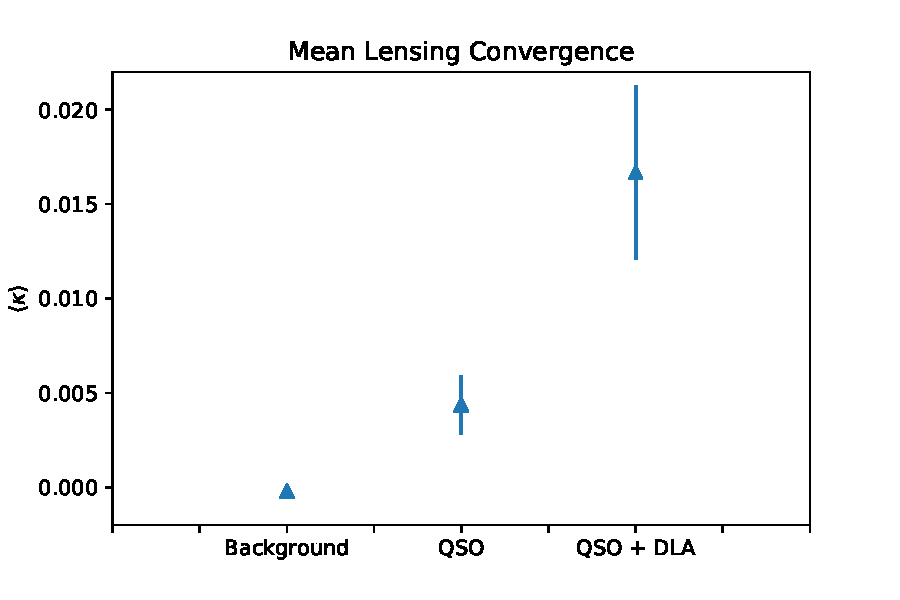
\includegraphics[width=\linewidth]{weighted.pdf}
  \caption{Mean weighted values of lensing convergence ($\kappa$) (from Planck map) for the entire sky and Quasars and DLAs (from BOSS DR12). The quasars are weighted to match the redshift distribution of the Quasars associated with DLAs. The QSO error is computed using bootstrap resampling. $\langle\kappa\rangle_{back} =-2 \times 10^{-4} \pm 8 \times 10^{-5}  , \langle\kappa\rangle_{qso} = 0.0044 \pm 0.0016, \langle\kappa\rangle_{dla} = 0.0167 \pm 0.0046$  }
  \label{fig:kmean}

  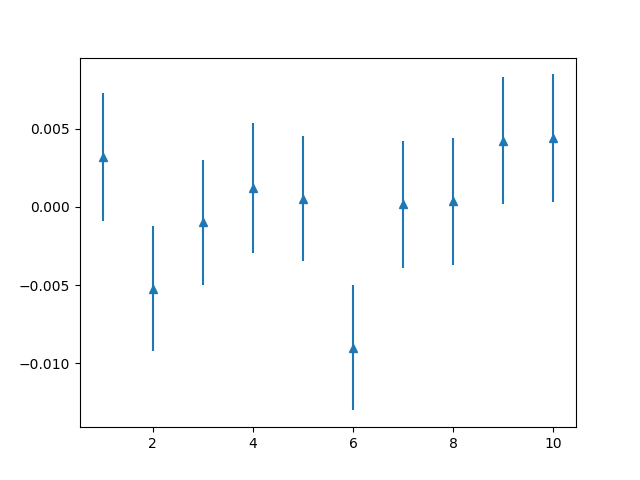
\includegraphics[width=\linewidth]{testfig.png}
  \caption{Ten trials finding the lensing convergence ($\kappa$) (from Planck map) for a random sample of points (within the kappa mask) the same size as the sample of DLAs. This confirms the error in Figure \ref{fig:kmean}.}
  \label{fig:ktest}
\end{figure}


\begin{figure}
  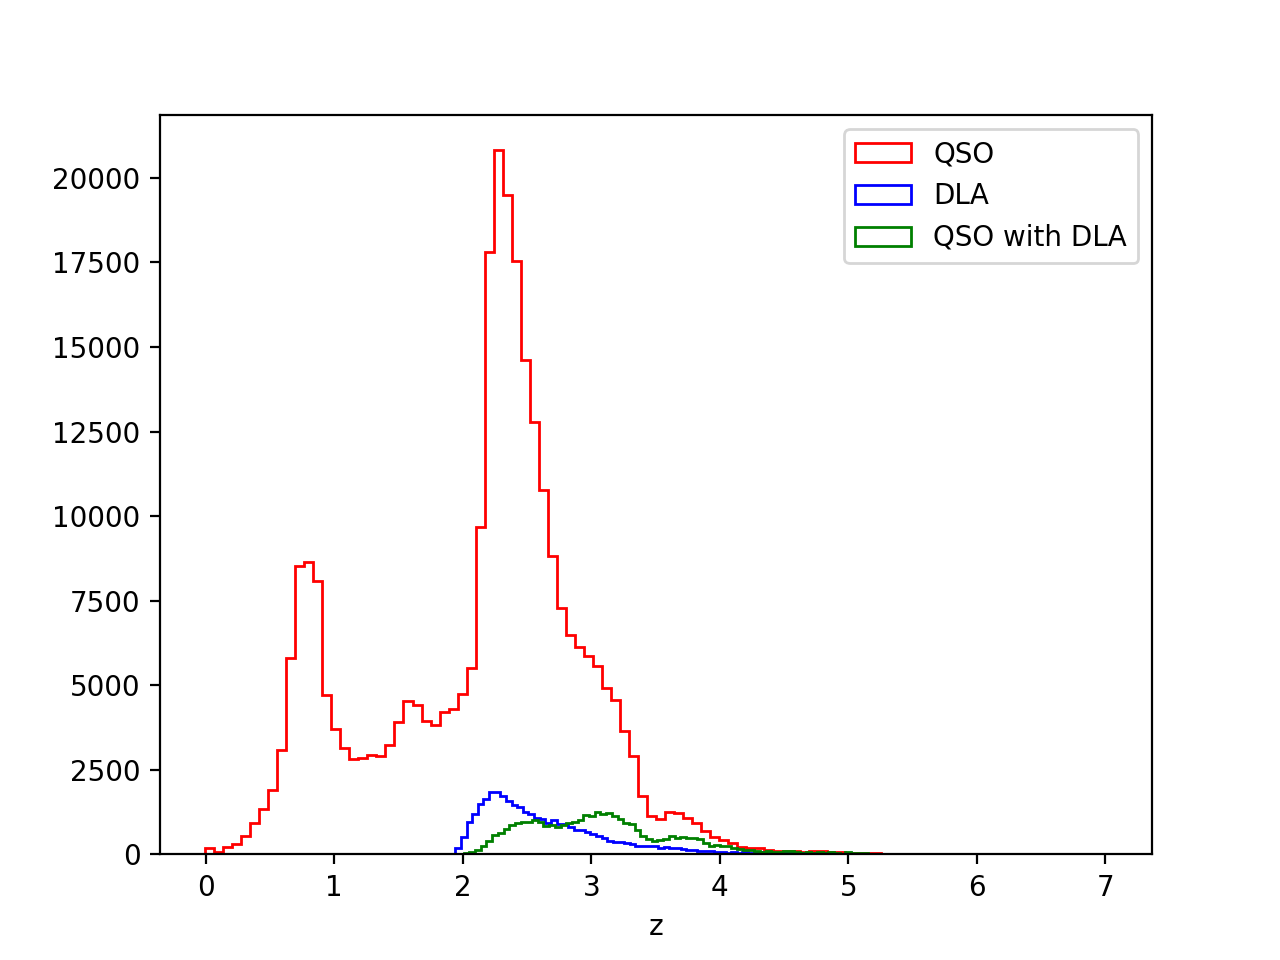
\includegraphics[width=\linewidth]{redshift.png}
  \caption{Redshift distribution of QSOs and DLAs with associated QSOs from BOSS DR12. Used in CCL to predict the cross power spectrum.}
  \label{fig:redshift}
  
    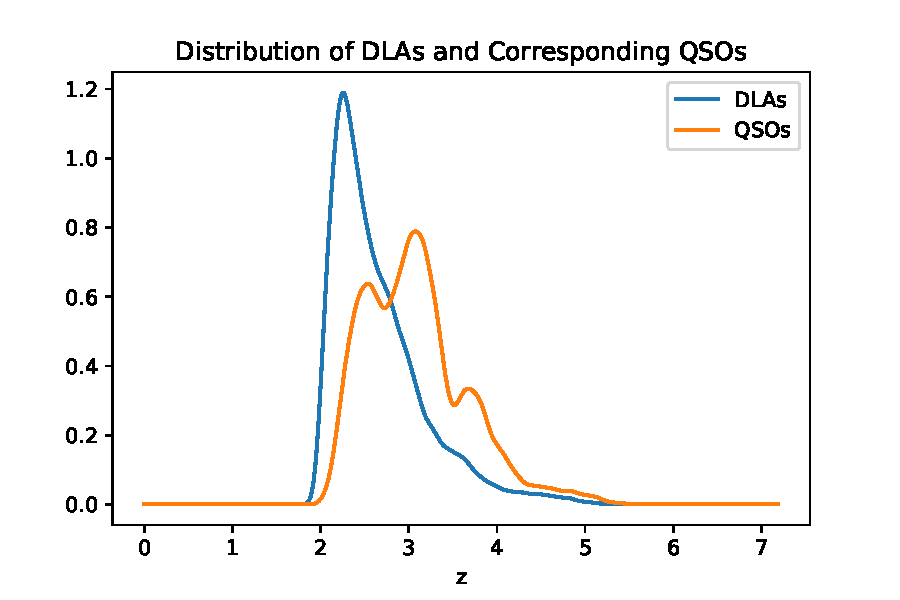
\includegraphics[width=\linewidth]{rdshift_ccl.pdf}
  \caption{Redshift distribution of DLAs with associated QSOs (smooth normalized version of small curves in Fig \ref{fig:redshift}). Used in CCL to predict the cross power spectrum. Produced using scipy.stats.gaussian\_kde}
  \label{fig:rdshift}
\end{figure}

\begin{figure}
  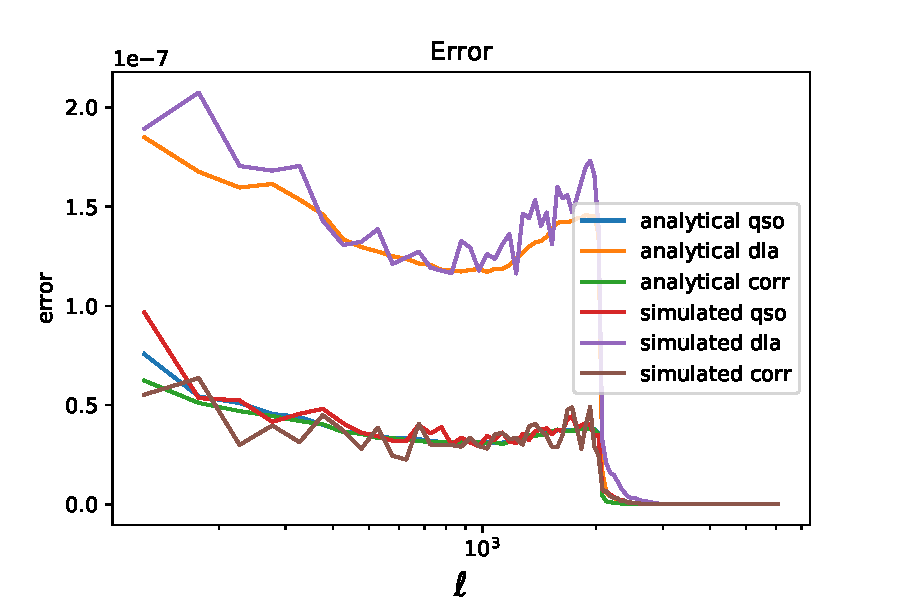
\includegraphics[width=\linewidth]{error_both.pdf}
  \caption{The error for QSOs, DLAs, and the covariance computed analytically as well as computed using the Planck simulations.}
  \label{fig:error}

  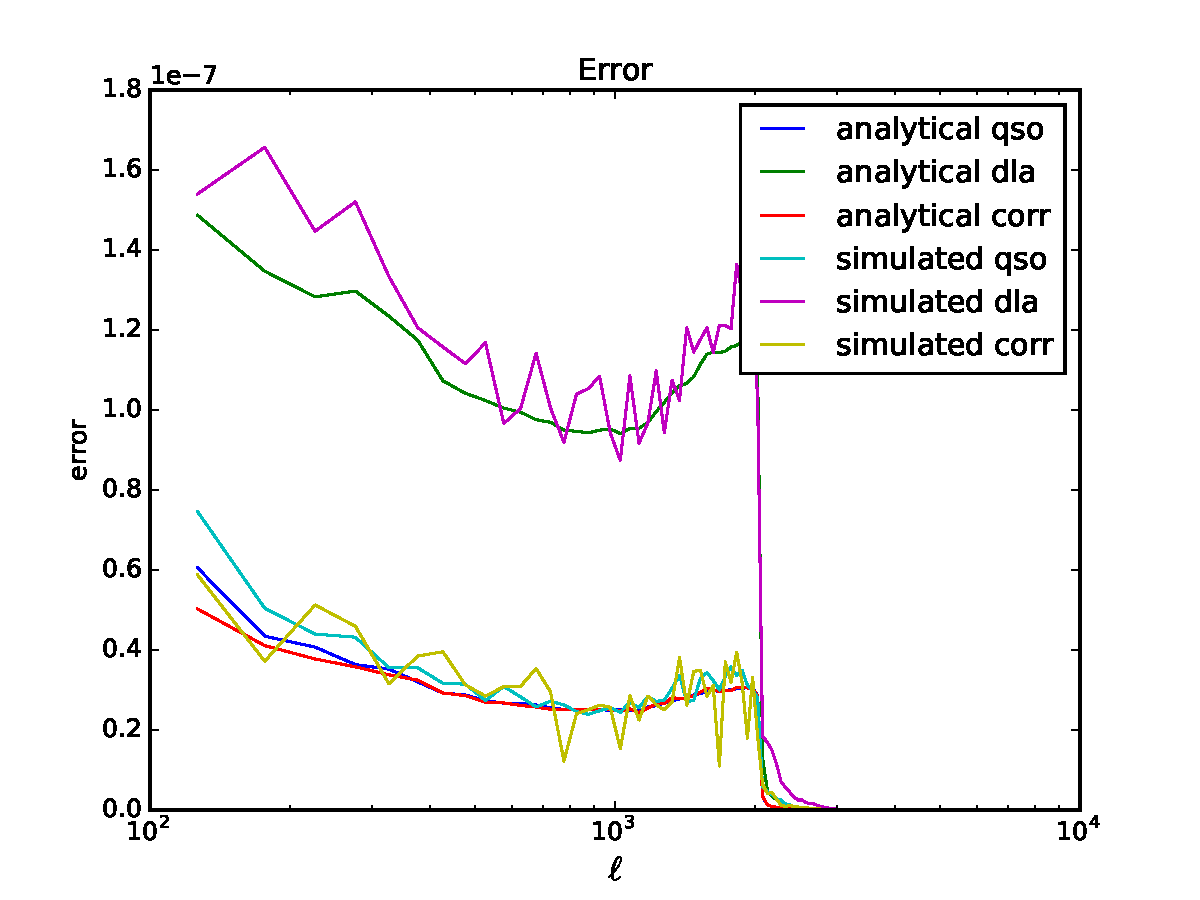
\includegraphics[width=\linewidth]{error_both_syn.pdf}
  \caption{The error for QSOs, DLAs, and the covariance computed analytically as well as computed using the 100 synfast simulations used to find the biasses in tables 4-6.}
  \label{fig:errorsyn}
\end{figure}

\begin{figure}
  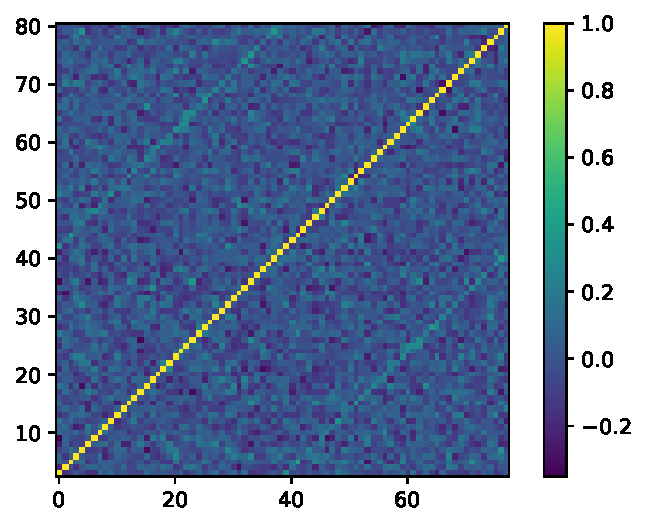
\includegraphics[width=\linewidth]{covariance.pdf}
  \caption{The covariance matrix where the first 40 bins are for the QSO cross power spectrum with the simulations and the last 40 are those for DLAs. This image was produced using 100 simulations with bins of 50 ells.}
  \label{fig:convariance}
\end{figure}

\begin{figure}
  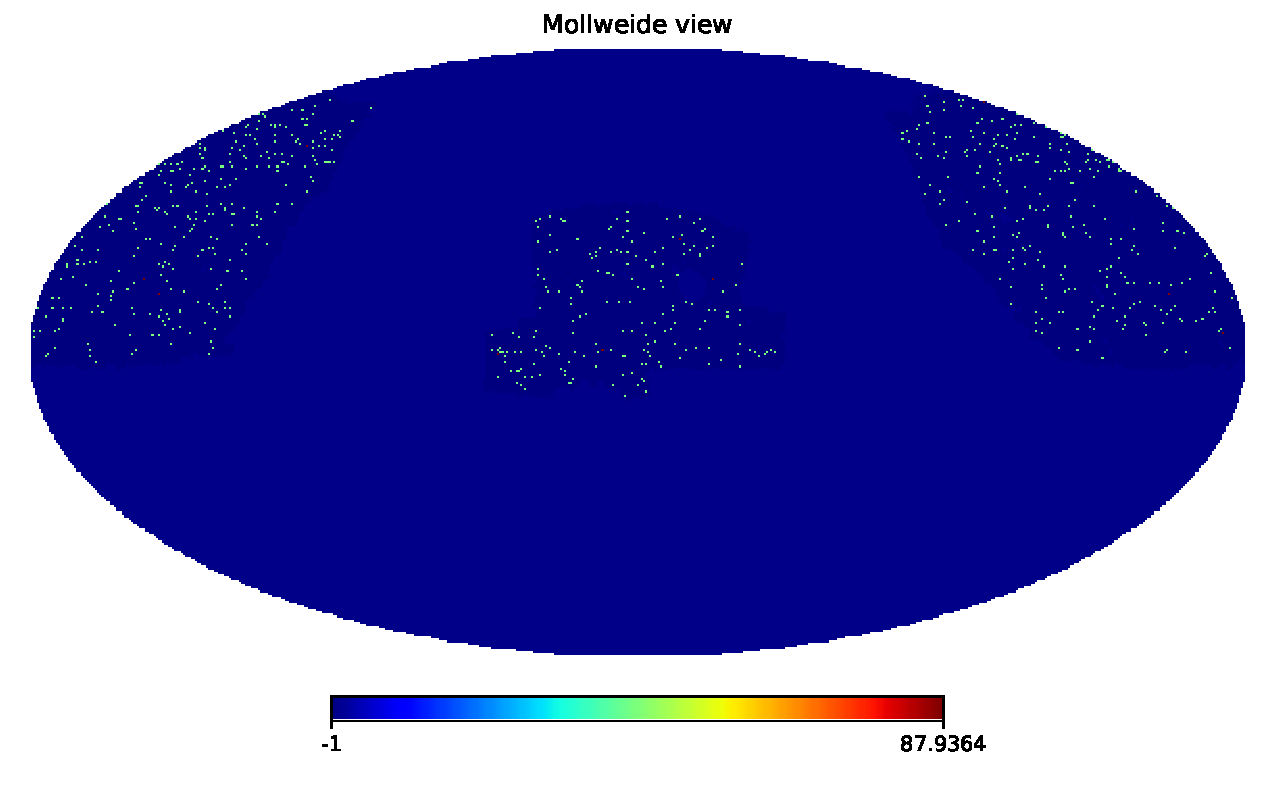
\includegraphics[width=\linewidth]{qso_map.pdf}
  \caption{Healpix map (Nside = 2048) of density of QSOs relative to the mean density in the area covered by the mask (the area outside the mask is set to zero). This is the map used with the Planck map to compute the cross power spectrum. The same method is used to create the DLA map. This map is in celestial coordinates. }
  \label{fig:qsomap}

  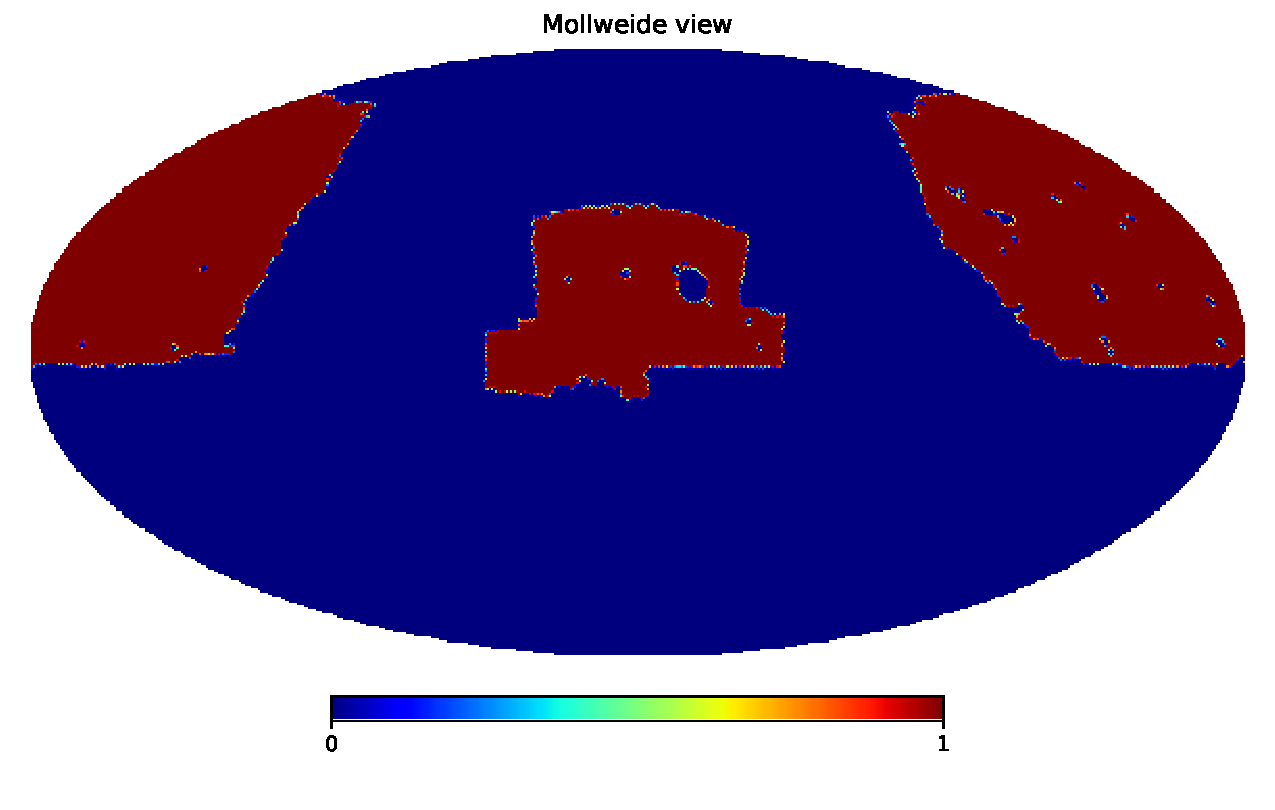
\includegraphics[width=\linewidth]{qso_mask.pdf}
  \caption{Mask of area used in computing the power spectrum. Created by degrading map to nside=64 and selecting pixels with QSOs then upgrading back to nside =2048. The map was smoothed using pymaster.mask$\_$apodization with 0.1 degree smoothing. The same method was used to create the DLA mask. }
  \label{fig:qsomask}
\end{figure}

\begin{figure}
  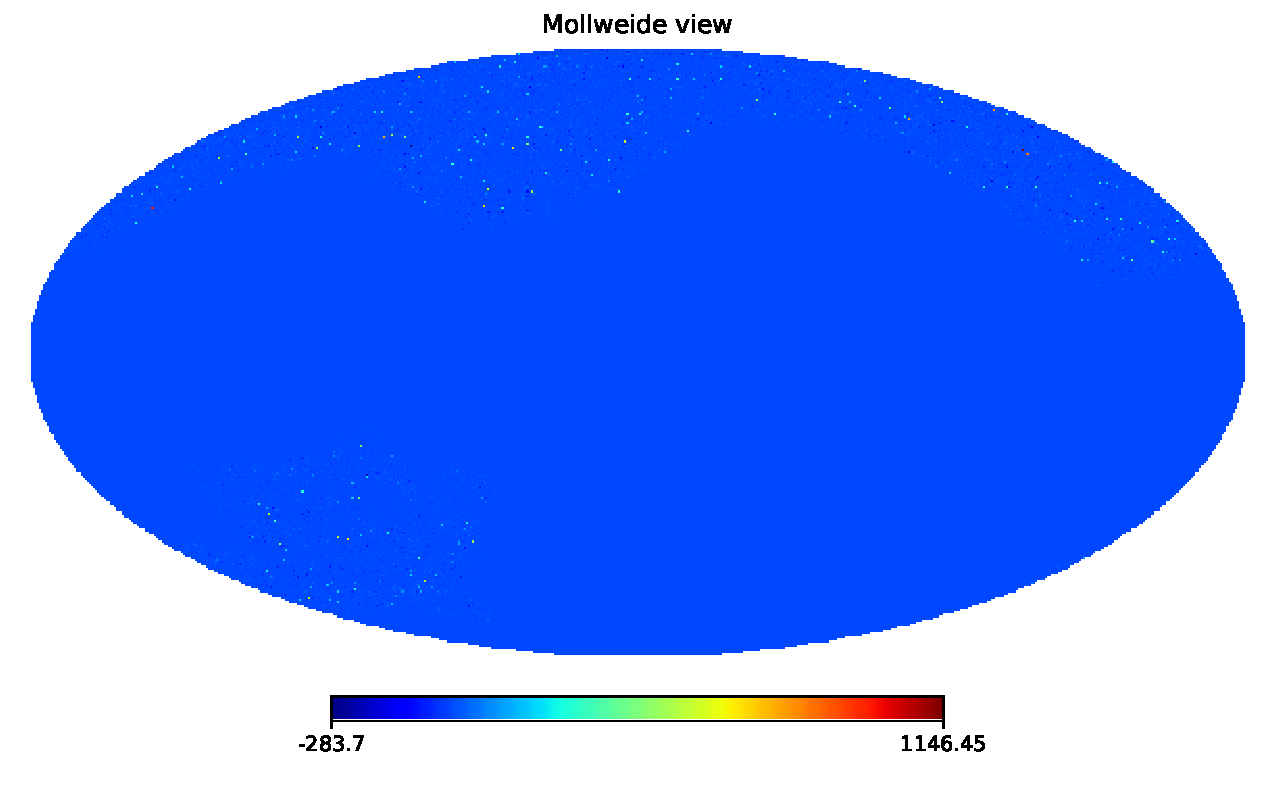
\includegraphics[width=\linewidth]{dla_map.pdf}
  \caption{Healpix map (Nside = 2048) of density of DLAs relative to the mean density in the area covered by the mask (the area outside the mask is set to zero). This is the map used with the Planck map to compute the cross power spectrum. This map was rotated into galactic coordinates using healpy.rotate$\_$alm. }
  \label{fig:dlamap}
\break \indent \break
  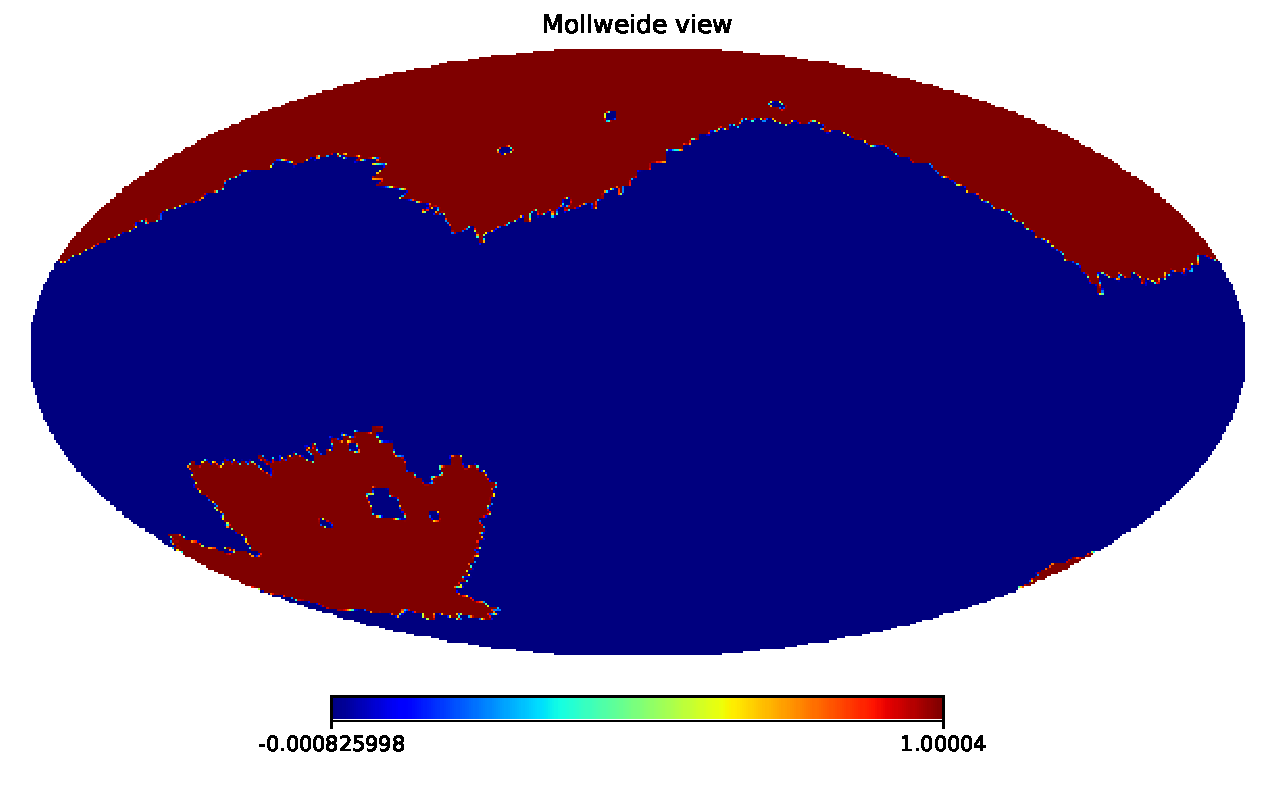
\includegraphics[width=\linewidth]{dla_mask.pdf}
  \caption{Mask of area used in computing the power spectrum. This mask was rotated from celestial to galactic coordinates using healpy.rotate$\_$alm. }
  \label{fig:dlamask}
\end{figure}

\begin{figure}
  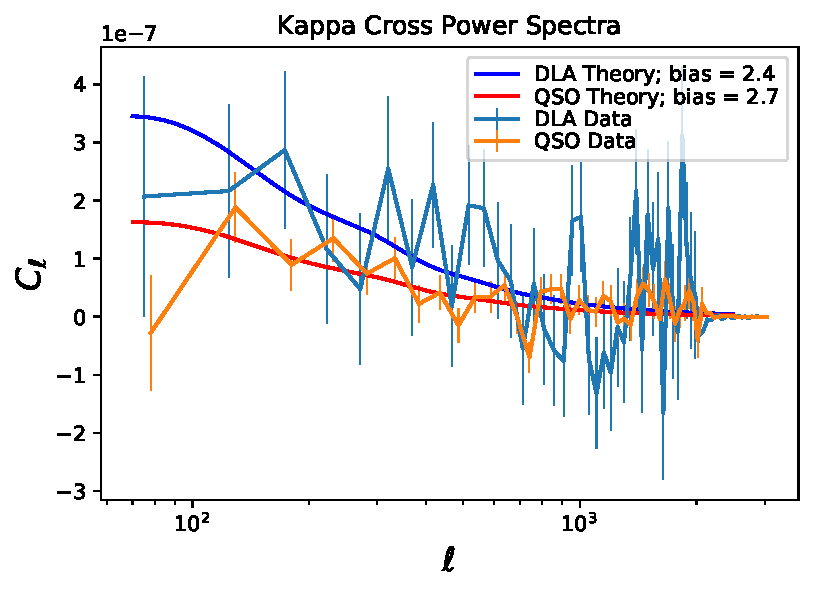
\includegraphics[width=\linewidth]{cps_predictions_50.pdf}
  \caption{The cross power spectrum of lensing convergence with DLAs and QSOs. The actual power spectra were computed using NaMaster, while the theoretical power spectra were computed using CCL (and the redshift distribution of DLAs and QSOs with DLAs from Fig \ref{fig:rdshift}). The values of the bias were selected by maximizing the log likelihood using scipy.optimize.minimize.}
  \label{fig:cpsdla}
\end{figure}

\begin{table}[htbp]
\caption{Bias with minimum $\chi^2$  for different $\ell_{max}$ using 25 $\ell$'s per bin using 100 hp.synfast sims.}
\centering
\begin{tabular}{p{0.18\textwidth}p{0.18\textwidth}p{0.18\textwidth}p{0.18\textwidth}p{0.18\textwidth}p{0.18\textwidth}} \\ \toprule
$\ell_{max}$ & \multicolumn{1}{p{0cm}}{$b_{QSO}$} & $b_{DLA}$ & \multicolumn{1}{p{2cm}}{$\chi^2$} & d.o.f  & Probability\\ \midrule
300  &  3.08  $\pm$  0.73  &  1.37  $\pm$  1.47  &  13.18  &  22  &  0.07 \\
600  &  2.81  $\pm$  0.54  &  2.3  $\pm$  1.24  &  29.27  &  46  &  0.03 \\
900  &  2.76  $\pm$  0.51  &  2.37  $\pm$  1.2  &  64.83  &  70  &  0.35 \\
1200  &  2.86  $\pm$  0.5  &  2.26  $\pm$  1.19  &  88.37  &  94  &  0.36 \\
1500  &  2.92  $\pm$  0.49  &  2.2  $\pm$  1.19  &  112.87  &  118  &  0.38 \\
1800  &  2.98  $\pm$  0.49  &  2.22  $\pm$  1.19  &  136.44  &  142  &  0.38 \\
2100  &  3.04  $\pm$  0.49  &  2.23  $\pm$  1.18  &  157.83  &  166  &  0.34 \\ \bottomrule
\end{tabular}
\vspace{2cm}
\caption{Bias with minimum $\chi^2$  for different $\ell_{max}$ using 50 $\ell$'s per bin using 100 hp.synfast sims.}
\centering
\begin{tabular}{p{0.18\textwidth}p{0.18\textwidth}p{0.18\textwidth}p{0.18\textwidth}p{0.18\textwidth}p{0.18\textwidth}} \\ \toprule
$\ell_{max}$ & \multicolumn{1}{p{0cm}}{$b_{QSO}$} & $b_{DLA}$ & \multicolumn{1}{p{2cm}}{$\chi^2$} & d.o.f  & Probability\\ \midrule
300  &  3.18  $\pm$  0.65  &  1.23  $\pm$  1.45  &  8.26  &  10  &  0.4 \\
600  &  2.9  $\pm$  0.49  &  2.11  $\pm$  1.21  &  17.82  &  22  &  0.28 \\
900  &  2.76  $\pm$  0.51  &  2.37  $\pm$  1.2  &  64.83  &  70  &  0.35 \\
1200  &  2.86  $\pm$  0.46  &  2.26  $\pm$  1.15  &  52.62  &  46  &  0.77 \\
1500  &  2.87  $\pm$  0.45  &  2.23  $\pm$  1.14  &  61.09  &  58  &  0.63 \\
1800  &  2.92  $\pm$  0.45  &  2.26  $\pm$  1.14  &  76.64  &  70  &  0.73 \\
2100  &  2.94  $\pm$  0.45  &  2.3  $\pm$  1.14  &  87.64  &  82  &  0.69 \\ \bottomrule
\end{tabular}


\vspace{2cm}
\caption{Bias with minimum $\chi^2$  for different $\ell_{max}$ using 75 $\ell$'s per bin using 100 hp.synfast sims.}
\centering
\begin{tabular}{p{0.18\textwidth}p{0.18\textwidth}p{0.18\textwidth}p{0.18\textwidth}p{0.18\textwidth}p{0.18\textwidth}} \\ \toprule
$\ell_{max}$ & \multicolumn{1}{p{0cm}}{$b_{QSO}$} & $b_{DLA}$ & \multicolumn{1}{p{2cm}}{$\chi^2$} & d.o.f  & Probability\\ \midrule
300  &  3.33  $\pm$  0.85  &  1.74  $\pm$  1.6  &  7.15  &  6  &  0.69 \\
600  &  3.01  $\pm$  0.54  &  2.36  $\pm$  1.29  &  14.85  &  14  &  0.61 \\
900  &  2.87  $\pm$  0.5  &  2.76  $\pm$  1.24  &  30.09  &  22  &  0.88 \\
1200  &  2.99  $\pm$  0.49  &  2.47  $\pm$  1.23  &  54.88  &  30  &  1.0 \\
1500  &  3.04  $\pm$  0.49  &  2.27  $\pm$  1.22  &  64.25  &  38  &  1.0 \\
1800  &  3.1  $\pm$  0.49  &  2.34  $\pm$  1.22  &  72.38  &  46  &  0.99 \\
2100  &  3.11  $\pm$  0.49  &  2.4  $\pm$  1.22  &  77.6  &  54  &  0.98 \\ \bottomrule
\end{tabular}
\end{table}



\end{document}